\section{Bắt đầu: mở Fiji và chuẩn bị ba ảnh kiểm chứng}
\label{sec:fiji-start}
Phần thực hành này dùng chính kết quả mẫu đã chạy thành công bằng Python. Mục tiêu là tự thao tác trong Fiji, nhìn thấy ảnh đầu vào và nhận được một ảnh nhãn do MorphoLibJ tính, sau đó đo kết quả bằng nhãn đúng. Không cần mở ứng dụng MorphoLab.

\begin{figure}[htbp]\centering
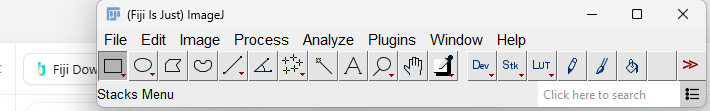
\includegraphics[width=0.94\linewidth]{figures/fiji_toolbar.png}
\caption{Cửa sổ thanh công cụ Fiji/ImageJ trong lần cài đặt trên máy người học. File dùng mở/lưu ảnh; Plugins chứa MorphoLibJ; mỗi ảnh có cửa sổ riêng.}\label{fig:fiji-toolbar}
\end{figure}

\begin{enumerate}[leftmargin=*,itemsep=4pt]
\item Mở \texttt{C:\textbackslash Tools\textbackslash Fiji\textbackslash fiji-windows-x64.exe}. Fiji có cửa sổ thanh công cụ nhỏ, không phải một cửa sổ làm việc toàn màn hình. Ảnh mở ra trong các cửa sổ riêng.
\item Kiểm tra menu \textbf{Plugins $\to$ MorphoLibJ}. Nếu chưa có, vào \textbf{Help $\to$ Update $\to$ Manage update sites}, bật \textbf{IJPB-plugins}, áp dụng cập nhật và mở lại Fiji. Máy thực nghiệm đã có MorphoLibJ 1.6.5.
\item Trong Anaconda Prompt đã kích hoạt env \texttt{ai}, chạy lệnh dưới đây một lần để tạo đúng dữ liệu kiểm chứng. Nếu đã chạy và có đủ tệp, chuyển sang bước tiếp theo.
\end{enumerate}
\begin{lstlisting}[language={},numbers=none]
cd /d D:\XU_LY_ANH
python -m morpholab segment data\synthetic\synth_00.tif ^
 --truth data\synthetic\synth_00_gt.tif ^
 --out outputs\demo_shared --fiji
\end{lstlisting}

Trong Fiji chọn \textbf{File $\to$ Open} hoặc \textbf{Ctrl+O}, mở lần lượt ba tệp trong thư mục \texttt{D:\textbackslash XU\_LY\_ANH\textbackslash outputs\textbackslash demo\_shared\textbackslash fiji}. Chỉ cần mở ba ảnh này trước khi chạy Watershed.

\begin{table}[htbp]\centering\small
\caption{Ba đầu vào của Watershed trong phép kiểm chứng chung dữ liệu.}\label{tab:fiji-inputs}
\begin{tabularx}{\linewidth}{l X X}\toprule
Tệp & Ý nghĩa & Cách đọc hình \\\midrule
\texttt{elevation.tif} & Địa hình $E=-D$, giá trị thực 32-bit & Tâm vật thể là vùng thấp; không đổi dấu hay chuẩn hóa lại.\\
\texttt{markers.tif} & Nhãn các hạt giống, nền bằng 0 & Mỗi ID dương khởi tạo một vùng; ảnh có thể tối vì ID chỉ 1--7.\\
\texttt{mask.tif} & Miền tiền cảnh được phép lan nhãn & Trắng là đối tượng; đen là nền.\\\bottomrule
\end{tabularx}\end{table}

\section{Chạy bằng menu Marker-controlled Watershed}
\label{sec:fiji-menu}
\begin{enumerate}[leftmargin=*,itemsep=5pt]
\item Chọn \textbf{Plugins $\to$ MorphoLibJ $\to$ Segmentation $\to$ Marker-controlled Watershed}. Có thể tìm tên lệnh bằng ô tìm kiếm Fiji khi menu thay đổi theo phiên bản.
\item Trong hộp thoại, chọn \textbf{Input = elevation.tif}, \textbf{Marker = markers.tif}, \textbf{Mask = mask.tif}. Không chọn ảnh gốc làm Marker.
\item Với MorphoLibJ 1.6.5, bỏ tích \textbf{Use diagonal connectivity} để dùng liên thông 4 trong ảnh 2D; bật ô này tương ứng liên thông 8. Đặt \textbf{Compactness = 0}. Bỏ \textbf{Binary markers} vì \texttt{markers.tif} đã chứa ID nhãn. Bỏ \textbf{Calculate dams}: phép so sánh đang dùng không tạo đường phân cách mang nhãn nền. Nếu phiên bản khác hiển thị một danh sách Connectivity, chọn 4.
\item Bấm \textbf{OK}. Fiji tạo một ảnh nhãn mới. Với ví dụ này, kết quả mong đợi là \textbf{7 đối tượng}. Màu hoặc số ID không nhất thiết trùng Python; không so hai ảnh chỉ bằng màu.
\item Nếu kết quả gần như đen, đổi \textbf{Image $\to$ Lookup Tables} sang một LUT màu hoặc chỉnh \textbf{Image $\to$ Adjust $\to$ Brightness/Contrast}. Chỉ thay cách hiển thị. Giữ ảnh nhãn số nguyên/thực chứa ID khi lưu, không chuyển sang RGB để chấm điểm.
\item Chọn \textbf{File $\to$ Save As $\to$ Tiff}, lưu tên \texttt{fiji\_manual\_labels.tif} trong thư mục trên. Tên khác được phép nếu thay đúng đường dẫn ở lệnh đánh giá.
\end{enumerate}

\section{Lưu kết quả và đo định lượng}
\label{sec:fiji-measure}
Sau khi lưu ảnh nhãn từ Fiji, quay lại Anaconda Prompt:
\begin{lstlisting}[language={},numbers=none]
python -m morpholab evaluate ^
 data\synthetic\synth_00_gt.tif ^
 outputs\demo_shared\fiji\fiji_manual_labels.tif ^
 --out outputs\demo_shared\fiji\manual_metrics.json
\end{lstlisting}
Mở \texttt{manual\_metrics.json}. Kỳ vọng \texttt{predicted\_objects=7}, \texttt{true\_objects=7}, \texttt{object\_f1=1}. IoU tiền cảnh xấp xỉ 0,981397 và Dice xấp xỉ 0,990611. Đây là điểm của ảnh ví dụ; bảng ảnh thật ở Chương~\ref{chap:experiments} mới dùng để đánh giá quy mô nhiều ảnh.

Phía Fiji/Java còn tự tính IoU, Dice và số đối tượng vào \texttt{fiji\_metrics.csv}. Mở tệp này cạnh \texttt{metrics.json} của Python để thấy phép đo trên cả hai nền tảng. Giá trị đồng thuận Python--Fiji khoảng 0,9848 trên ví dụ là độ giống nhau sau ghép ID, khác với F1 so với nhãn đúng. Fiji không được coi là ground truth.

Có thể xem thuộc tính nhãn bằng nhóm lệnh \textbf{Plugins $\to$ MorphoLibJ $\to$ Analyze} rồi chọn lệnh phân tích vùng 2D tương ứng. Chọn ảnh nhãn đầu vào để đọc số vùng/diện tích. Các đại lượng hình học phụ thuộc chuẩn liên thông, phép đo chu vi và hiệu chuẩn pixel, vì vậy muốn đối chiếu phải dùng cùng đơn vị. Với thí nghiệm này diện tích báo theo pixel$^2$. Không dùng \textbf{Analyze Particles} trên mask chưa tách để thay số nhãn Watershed: hai vật chạm nhau có thể bị đếm chung.

\section{Chạy lại bằng script Groovy tự động}
\begin{enumerate}[leftmargin=*]
\item Trong Fiji mở \textbf{File $\to$ New $\to$ Script}; chọn \textbf{Language = Groovy}.
\item Mở tệp \texttt{outputs/demo\_shared/fiji/Run\_in\_Fiji.groovy} trong editor. Tệp này có sẵn đường dẫn tuyệt đối đến ba ảnh của lần chạy.
\item Bấm \textbf{Run}. Một ảnh nhãn hiện ra và tệp \path{fiji_interactive_labels.tif} được lưu cạnh các đầu vào.
\item Dùng lệnh \texttt{evaluate} như trên, thay tên dự đoán thành \path{fiji_interactive_labels.tif}. Kết quả cần tương ứng phép chạy menu nếu chọn cùng tham số.
\end{enumerate}
Script dùng chung \texttt{fiji/ReplayWatershed.groovy} có hộp chọn thư mục, liên thông 4/8 và bật/tắt hiển thị. Chọn thư mục có đủ ba TIFF như Bảng~\ref{tab:fiji-inputs}. Toàn bộ script ở phụ lục; phần tính toán đã được kiểm tra bằng Groovy với hiển thị tắt, không chỉ được viết để minh họa.

\section{Khảo sát các toán tử hình thái trong Fiji}
Để học phép toán trước khi chạy cả quy trình, mở \texttt{mask.tif}, tạo bản sao bằng \textbf{Image $\to$ Duplicate}, rồi tìm \textbf{Morphological Filters} trong nhóm \textbf{MorphoLibJ $\to$ Filtering}. Chọn lần lượt Erosion, Dilation, Opening, Closing trên \emph{các bản sao của cùng ảnh ban đầu}; chọn SE vuông, bán kính 1 để đối chiếu hình minh họa ở Chương~\ref{chap:theory}. Không chạy liên tiếp co rồi giãn trên cùng cửa sổ rồi nhầm đó là hai đầu ra độc lập.

Các lệnh reconstruction trong nhóm Filtering cho phép nhận marker và mask. Bản native tự động xuất \path{native_erosion.tif}, \path{native_dilation.tif}, \path{native_opening.tif}, \path{native_closing.tif} và \path{native_reconstruction.tif}; đây là bộ minh chứng cùng quy trình và tham số để so với thao tác tay.

\section{Nhật ký thực hành cần giữ}
Mỗi lần thực hành ghi tên ảnh, SE/h/radius/connectivity, tùy chọn dams, tên tệp kết quả và chỉ số. Nếu đếm sai, xem mask trước: mask rỗng thì Watershed không thể tạo lại vùng đã bị loại. Nếu còn mask nhưng chia thừa/gộp sai, xem marker và khoảng cách. Hình giao diện Fiji trong báo cáo là minh chứng thao tác; nhãn TIFF và CSV mới là dữ liệu để đo và tái lập.
